\section{Results}
\label{sec:results}

This section describes the significance of collecting
run time application I/O event data using our \Darshan{} approach. We present 
performance analyses that show how the new metrics, captured in a time series
along with \emph{absolute timestamps}, can provide more insight
into I/O behavior than summary statistics alone. 
%and how this information represented metrics intervals. 
Additionally, such representation
% using the absolute timestamps
can facilitate the correlation of I/O performance with system component
behaviors
(e.g., network and filesystem congestion)
% for example, with system behavior monitoring, 
which can also be represented in a Grafana dashboard.

Without the \connector{}, it would not be possible to create the meaningful analyses 
and visualizations shown in Figures\ref{f:mpi_io_all}-\ref{f:mpi_io_grafana}. 
In contrast, Figure~\ref{f:hacc2} shows the aggregate I/O behavior which can be 
created with Darshan alone. This figure does not provide the timeseries data and 
thus in-depth insights into I/O behavior like the \Darshan{} does. Note that
the Darshan eXtended Trace (DXT) plugin that we leverage in this work does provide
time series capture capability. However, due to memory constraints it will not 
typically be able to capture these time series for a whole job run. Additionally
the timestamps in the DXT time series are relative to the job start rather than
absolute.
%\section{Results}
%\label{sec:results}

%This section prsents the significance of our approach to collect
%runtime application I/O data using \Darshan{}. We present performance
%analysis that shows how the new metrics helped provide more insight
%results into I/O behavior and how this information represented
%in Grafana.

\subsection{Experiments and Overhead}
Each application was tested on both the Lustre and the NFS file system with 
several configurations for each application run. All application experiments 
were repeated 5 times for both the \connector{} and Darshan 
only (i.e. no LDMS implementation) scenarios. In total there were 40 experiments
run with a separate job submission for each. The details of these runs are shown 
in Table~\ref{table:apps}.  

\begin{table}[h]
    \begin{subtable}[h]{0.5\textwidth}
    \vspace{0.5cm}
        \centering
        \setlength\tabcolsep{8pt}
       \begin{tabular}{|ccccc|}
        \hline
        \multicolumn{5}{|c|}{MPI-IO-TEST}                                                                                                           \\ \hline
        \multicolumn{1}{|c|}{File System}     & \multicolumn{2}{c|}{NFS}                                    & \multicolumn{2}{c|}{Lustre}           \\ \hline
        \multicolumn{1}{|c|}{Nodes}           & \multicolumn{2}{c|}{22}                                     & \multicolumn{2}{c|}{22}               \\ \hline
        \multicolumn{1}{|c|}{Block Size}      & \multicolumn{2}{c|}{16*1024*1024}                           & \multicolumn{2}{c|}{16*1024*1024}     \\ \hline
        \multicolumn{1}{|c|}{Iterations}      & \multicolumn{2}{c|}{10}                                     & \multicolumn{2}{c|}{10}               \\ \hline
        \multicolumn{1}{|c|}{Collective}      & \multicolumn{1}{c|}{Yes}     & \multicolumn{1}{c|}{No}      & \multicolumn{1}{c|}{Yes}    & No      \\ \hline
        \multicolumn{1}{|c|}{Avg. Messages}   & \multicolumn{1}{c|}{50390}   & \multicolumn{1}{c|}{6397}    & \multicolumn{1}{c|}{25770}  & 15676   \\ \hline
        \multicolumn{1}{|c|}{Rate (msgs/sec)} & \multicolumn{1}{c|}{37}      & \multicolumn{1}{c|}{7}       & \multicolumn{1}{c|}{95}     & 38      \\ \hline
        \multicolumn{5}{|c|}{Average Runtime(s)}                                                                                                    \\ \hline
        \multicolumn{1}{|c|}{Darshan}         & \multicolumn{1}{c|}{1376.67} & \multicolumn{1}{c|}{880.46}  & \multicolumn{1}{c|}{249.97} & 428.18  \\ \hline
        \multicolumn{1}{|c|}{dC}              & \multicolumn{1}{c|}{1355.35} & \multicolumn{1}{c|}{858.68}  & \multicolumn{1}{c|}{270.98} & 414.35  \\ \hline
        \multicolumn{1}{|c|}{\% Overhead}     & \multicolumn{1}{c|}{-1.55\%} & \multicolumn{1}{c|}{-2.47\%} & \multicolumn{1}{c|}{8.41\%} & -3.23\% \\ \hline
        \multicolumn{5}{|c|}{Standard Deviation(s)}                                                                                                 \\ \hline
        \multicolumn{1}{|c|}{Darshan}         & \multicolumn{1}{c|}{48.18}   & \multicolumn{1}{c|}{29.43}   & \multicolumn{1}{c|}{2.85}   & 31.49   \\ \hline
        \multicolumn{1}{|c|}{dC}              & \multicolumn{1}{c|}{96.63}   & \multicolumn{1}{c|}{76.58}   & \multicolumn{1}{c|}{1.07}   & 8.17    \\ \hline
        \multicolumn{1}{|c|}{\% Variance}     & \multicolumn{1}{c|}{-5.25\%} & \multicolumn{1}{c|}{-8.10\%} & \multicolumn{1}{c|}{9.22\%} & 2.39\%  \\ \hline
        \end{tabular}
    \caption{MPI-IO} 
    \label{subtable:mpi-io-test}
    \vspace{0.5cm}
    \end{subtable}
    \begin{subtable}[h]{0.5\textwidth}
        \centering
        \setlength\tabcolsep{5.5pt}
        \begin{tabular}{|ccccc|}
        \hline
        \multicolumn{5}{|c|}{HACC-IO}                                                                                                                    \\ \hline
        \multicolumn{1}{|c|}{File System}     & \multicolumn{2}{c|}{NFS}                                      & \multicolumn{2}{c|}{Lustre}              \\ \hline
        \multicolumn{1}{|c|}{Nodes}           & \multicolumn{2}{c|}{16}                                       & \multicolumn{2}{c|}{16}                  \\ \hline
        \multicolumn{1}{|c|}{Particles/Rank}  & \multicolumn{1}{c|}{5000000}  & \multicolumn{1}{c|}{10000000} & \multicolumn{1}{c|}{5000000}  & 10000000 \\ \hline
        \multicolumn{1}{|c|}{Avg. Messages}   & \multicolumn{1}{c|}{1663}     & \multicolumn{1}{c|}{1774}     & \multicolumn{1}{c|}{1995}     & 1711     \\ \hline
        \multicolumn{1}{|c|}{Rate (msgs/sec)} & \multicolumn{1}{c|}{2}        & \multicolumn{1}{c|}{1}        & \multicolumn{1}{c|}{3}        & 2        \\ \hline
        \multicolumn{5}{|c|}{Average Runtime(s)}                                                                                                        \\ \hline
        \multicolumn{1}{|c|}{Darshan}         & \multicolumn{1}{c|}{882.46}   & \multicolumn{1}{c|}{1353.87}  & \multicolumn{1}{c|}{417.14}   & 1616.87  \\ \hline
        \multicolumn{1}{|c|}{dC}              & \multicolumn{1}{c|}{775.24}   & \multicolumn{1}{c|}{1365.24}  & \multicolumn{1}{c|}{467.24}   & 1027.44  \\ \hline
        \multicolumn{1}{|c|}{\% Overhead}     & \multicolumn{1}{c|}{-12.15\%} & \multicolumn{1}{c|}{0.84\%}   & \multicolumn{1}{c|}{12.01\%}  & -36.45\% \\ \hline
        \multicolumn{5}{|c|}{Standard Deviation(s)}                                                                                                         \\ \hline
        \multicolumn{1}{|c|}{Darshan}         & \multicolumn{1}{c|}{37.08}    & \multicolumn{1}{c|}{87.24}    & \multicolumn{1}{c|}{25.03}    & 154.53   \\ \hline
        \multicolumn{1}{|c|}{dC}              & \multicolumn{1}{c|}{53.68}    & \multicolumn{1}{c|}{46.97}    & \multicolumn{1}{c|}{142.77}   & 256.62   \\ \hline
        \multicolumn{1}{|c|}{\% Variance}     & \multicolumn{1}{c|}{-14.65\%} & \multicolumn{1}{c|}{4.08\%}   & \multicolumn{1}{c|}{-17.25\%} & -47.36\% \\ \hline
        \end{tabular}
    \caption{HACC-IO} 
    \label{subtable:HACC}
    \vspace{0.5cm}
    \end{subtable}
%    \begin{subtable}[h]{0.5\textwidth}
%        \centering
%        \setlength\tabcolsep{19pt}
%        \begin{tabular}{|cclcl|}
%        \hline
%        \multicolumn{5}{|c|}{HMMER}                                                                            \\ \hline
%        \multicolumn{1}{|c|}{File System}     & \multicolumn{2}{c|}{NFS}      & \multicolumn{2}{c|}{Lustre}    \\ \hline
%        \multicolumn{1}{|c|}{Nodes}           & \multicolumn{2}{c|}{1}        & \multicolumn{2}{c|}{1}         \\ \hline
%        \multicolumn{1}{|c|}{Input}           & \multicolumn{4}{c|}{Pfam-A.seed}                               \\ \hline
%        \multicolumn{1}{|c|}{Avg. Messages}   & \multicolumn{2}{c|}{3117342}  & \multicolumn{2}{c|}{4461738}   \\ \hline
%        \multicolumn{1}{|c|}{Rate (msgs/sec)} & \multicolumn{2}{c|}{1483}     & \multicolumn{2}{c|}{2396}      \\ \hline
%        \multicolumn{5}{|c|}{Average Runtime (s)}                                                              \\ \hline
%        \multicolumn{1}{|c|}{Darshan}         & \multicolumn{2}{c|}{749.88}   & \multicolumn{2}{c|}{135.40}    \\ \hline
%        \multicolumn{1}{|c|}{dC}              & \multicolumn{2}{c|}{2826.01}  & \multicolumn{2}{c|}{1863.98}   \\ \hline
%        \multicolumn{1}{|c|}{\% Overhead}     & \multicolumn{2}{c|}{276.86\%} & \multicolumn{2}{c|}{1276.67\%} \\ \hline
%        \end{tabular}
%    \caption{HMMER} 
%    \label{subtable:HMMER}
%\end{subtable}

\caption{Overview of each experiment configuration, target file system, average elapsed time(s) and standard deviation(s) from 5 runs, calculated overhead of LDMS and variance of the runs.}
\label{table:apps}
\end{table}
%\RED{Took another stab at this. FIX ANYTHING THAT DOESN'T MAKE SENSE. OR REMOVE IT ALL TOGETHER}.
The average of the 5 execution times (e.g., Average Runtime (s)) for Darshan and 
the \connector{} (dC in the table) was used to calculate the percent overhead of LDMS. 
Because of the system availability, the runtimes with Darshan were only performed 
and recorded 1-2 weeks before the experiments with the \connector{}. As seen from 
Table~\ref{subtable:mpi-io-test}, the overhead of LDMS on Darshans' MPI-IO-TEST 
benchmark for three experiments shows a decrease in overall runtime with the \connector{}. 
Since this is not feasible, the runtime improvement seen with the \connector{} is most 
likely due to the NFS and Lustre file systems performance variation where (and when) 
these experiments were performed. This behavior will be further investigated by conducting
a new set of randomized experiments during dedicated time on a system to minimize variability
due to competing applications and the effects of resource performance variations.
%As of this publication We have not re-run these tests 
%on a different 
%cluster or have had the opportunity to interleave the Darshan, and \connector{} 
%runs to mitigate any file system performance changes.

%Since the applications for Darshan and the \connector{} were run at different times, the file systems could have performed worse during the Darshan experiments and better during the \connector{} experiments creating an increase and decrease in overhead, respectively.  

%The other experiment on the Lustre file system with Collective enabled shows an overhead of less than 8.41\%, which is a minor overhead as this experiment has the highest rate of messages being sent per second to the LDMS Streams interface. 

The HACC-IO application, seen in Table~\ref{subtable:HACC} was similar to the MPI-IO-TEST 
benchmark regarding a shorter runtime with the \connector{} for both file systems. Again, 
this is most likely due to differences in Lustre and NFS file system loading during different
experiments. The other two experiments, NFS with 10 million particles and Lustre with 
5 million particles, show an overhead of 0.84\% and 12.01\%, respectively. The experiment 
with 0.84\% overhead indicates no significant effect on the applications runtime. 
In contrast, the experiment with 12.01\% overhead shows a longer runtime with the 
\connector{} which is most likely due to performance variation in both file systems 
which we will investigate in the near future. The variance across all experiments is 
so large that the performance overhead calculations are inconclusive. 

%inconclusive for each of the experiments are statistically significant to assume that the overhead of LDMS is likely due to factors outside of LDMS and therefore are inconclusive. Based on the current data we can't quantify the overhead but plan to investigate this further. we can not make any assumptions about the significant increases in overhead (e.g. MPI-IO collective using luster).

%The HMMER application, seen in Table~\ref{subtable:HACC} shows a significant increase in runtime with upwards of 270\% for NFS and 12000\% for Lustre where the user has to wait ~2x-12x longer for their application to finish. This, of course, is not ideal for the average user and the result of these high overhead percentages are due to the json message formatting. Additional tests have been performed without the sprintf() function to generate the json message (i.e. only LDMS Streams API is enabled and the \connector send function is called) and the average overhead was 0.37\%. This indicates that the increase in overhead is not due to LDMS but rather the formatting of the I/O event data from integers into strings. HMMER had an average of 3-4 million messages (i.e. Darshan I/O events) during a single run with a rate of 1-2k messages per second. HACC-IO and MPI-IO-TEST, on the other hand, had an average of 1-50K messages with rates of less than 100 messages per second. These are significantly lower than HMMER which is why no significant overhead was detected in the other application runs. 
%\RED{explain this in future work section: We observed a significant increase in total runtime from the \connector{} for short I/O applications with an approximate rate of 500,000 messages sent per second. This large volume of data being collected and sent causes an increase in runtime because of the json message formatting we added in the Darshan code. We ran experiments with and without the json formatting and the runtime will significantly increase.

%Darshan collects all I/O events of an application run and the \connector{} is implemented such that when Darshan detects an I/O event, the \connector{} will collect and format that current set of I/O metrics into a json message. In order to send a json message, all integers must be converted to strings and this conversion comes at a performance cost. Therefore, the more I/O intensive an application is and the shorter the runtime, the overhead will increase significantly and cause the runtime performance to drop. Since there is currently no other way to send I/O data as a json message to the LDMS Streams interface without converting the integers to strings, we must pay a performance cost. If this issue persists when the variance is not statistically significant, we plan to further develop the \Darshan{} framework to allow users to collect every \emph{n-th} I/O event detected by Darshan. This functionality will allow users to analyze a percentage of their applications I/O behavior during runtime without having to sacrifice runtime performance.}

%For the experiments that show a significant increase in overhead, this is due to the json message formatting. Darshan collects all I/O events of an application run and the \connector{} is implemented such that when Darshan detects an I/O event, the \connector{} will collect and format that current set of I/O metrics into a json message. In order to send a json message, all integers must be converted to strings and this conversion comes at a performance cost. Therefore, the more I/O intensive an application is and the shorter the runtime, the overhead will increase significantly and cause the runtime performance to drop (as seen in MPI-IO collective using luster). Since there is currently no other way to send I/O data as a json message to the LDMS Streams interface without converting the integers to strings, we must pay this performance cost. To overcome this issue, we plan to further develop the \Darshan{} framework to allow users to collect every \emph{n-th} I/O event detected by Darshan. This functionality will allow users to analyze a percentage of their applications I/O behavior during runtime without having to sacrifice runtime performance.     
%\RED{END OF THE SECTION I'VE ADDED - 6/26}


\subsection{Analysis and Grafana Output}
%Figure \ref{f:hacc} presents the mean number of I/O operations for
%each HACC application and the error bar considering 95\% confidence
%interval for the five jobs. This plot shows that even running at the
%same system and with the same configuration, the applications
%presented different I/O behavior. In fact, a single HPC application
%can have multiple unique I/O behavior that can degradate the
%performance of the application \cite{costa2021}. This I/O variation
%can also happen between allocated devices.
Figure \ref{f:hacc2} shows the number of I/O requests per node for close and 
open operations for two jobs using the same input for the HACC-IO application 
on Lustre using 10 million particles per rank. The root cause of this variation 
is under investigation as we would expect identical runs to have identical
behavior with respect to location and number of open and close events.

%\begin{figure}
%	\centering
	% 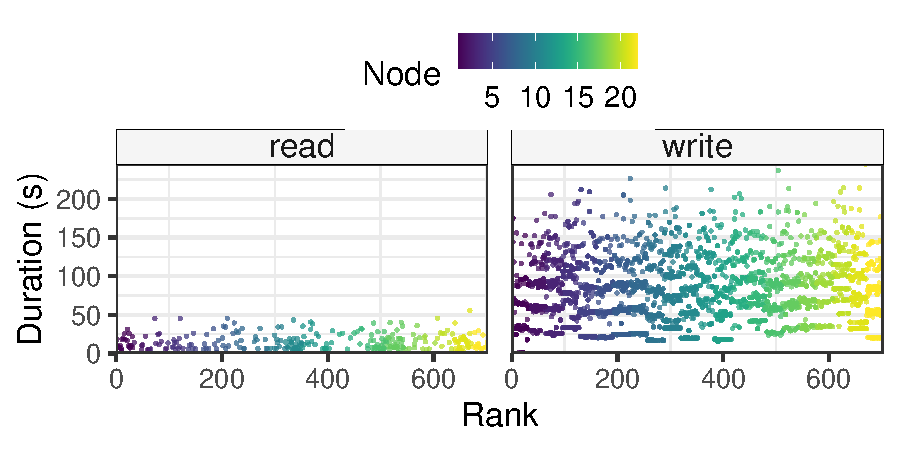
\includegraphics[width=\linewidth]{figs/255653_mpi_io_luster_no_coll_duration.pdf}
 %       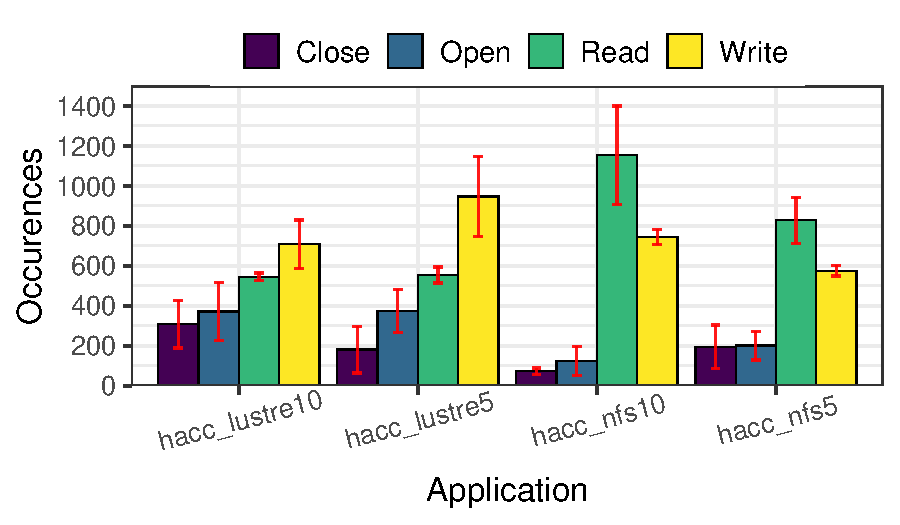
\includegraphics[width=1\linewidth]{figs/operations_hacc.pdf}
%	\caption{The same application can perform different amount of
%          I/O operations during execution. It shows the mean
%         occurrences of each operation over the five job runs.}
%	\label{f:hacc}
%\end{figure}

% jobs "255515", "255675"
\begin{figure}
	\centering
        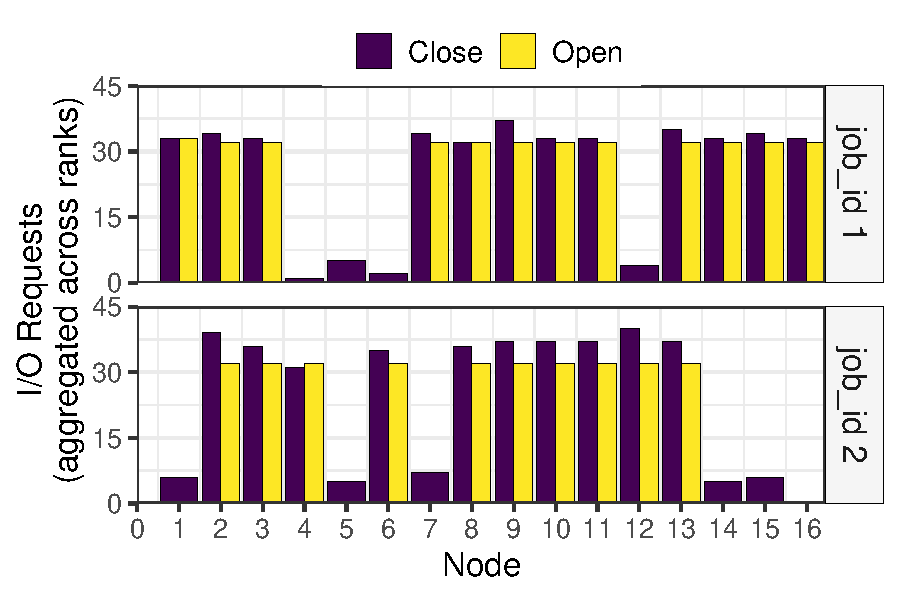
\includegraphics[width=\linewidth]{figs/hacc_nfs_10.pdf}
	\caption{The amount of I/O operations for HACC-IO using the same input.}
	\label{f:hacc2}
\end{figure}

Figure \ref{f:mpi_io_all} shows the duration of the reads and writes
per rank for each execution (\texttt{job\_id} metric) of the MPI-IO
benchmark without using collective operations. We notice a similar
behavior for the I/O operations duration for all jobs except the
second one (\texttt{job\_id 2}). It presents a mean duration of 6.75
seconds for reads and 78s for writes, while the other jobs had a mean
duration of 0.05s for reads and 54s for writes. With the collected
logs, we can perform a spatial performance analysis to understand the
variability in the I/O behavior per system component, in this case,
per node and rank.
      
\begin{figure}
	\centering
        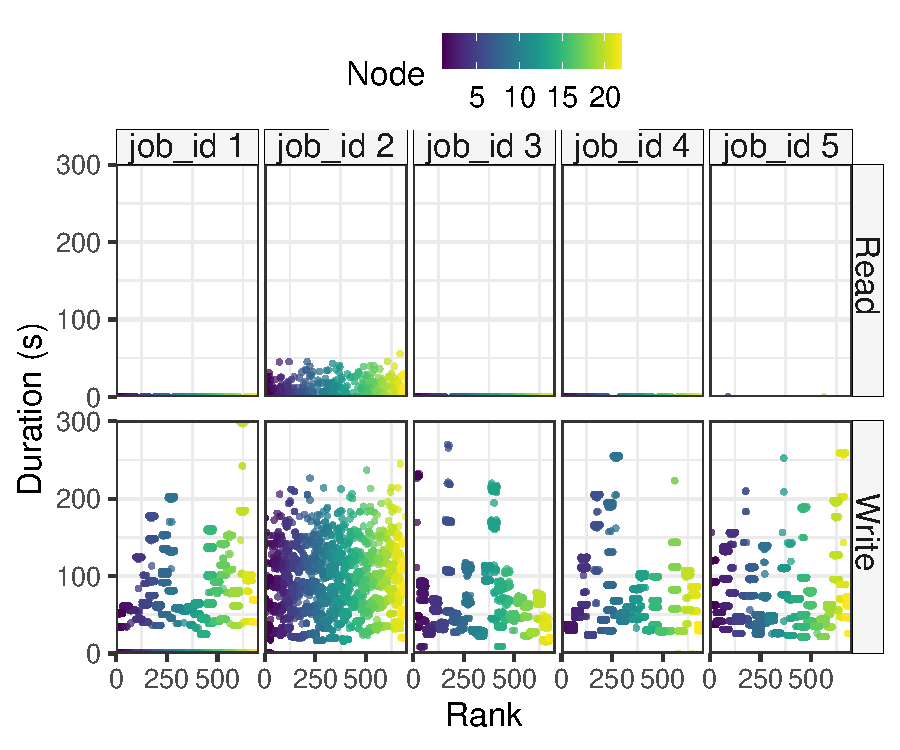
\includegraphics[width=\linewidth]{figs/mpi_io_luster_no_coll_duration_allexperiments.pdf}
	\caption{Jobs for the MPI-IO benchmark without collective
          operations presented variability in the number and duration
          of I/O operations.}
	\label{f:mpi_io_all}
\end{figure}

Using the absolute timestamps collected we can temporally view
where, in the application execution, the variability of a job
occurred and better understand the I/O behavior. 
Figure \ref{f:mpi_io} presents the duration and occurrence of
I/O operations throughout the MPI-IO benchmark for \texttt{job\_id
  2}. We can identify the application I/O pattern of performing
writes during the ten iterations, and the likewise the ten read iterations at the end
though these are smaller and less distinct than the writes. 
It can also be seen that in general writes became progressively slower over
the application execution time.
%application run faster writes at the beginning and slower at the end,
%with the slowest writing after 250 seconds.
      
\begin{figure}
	\centering
	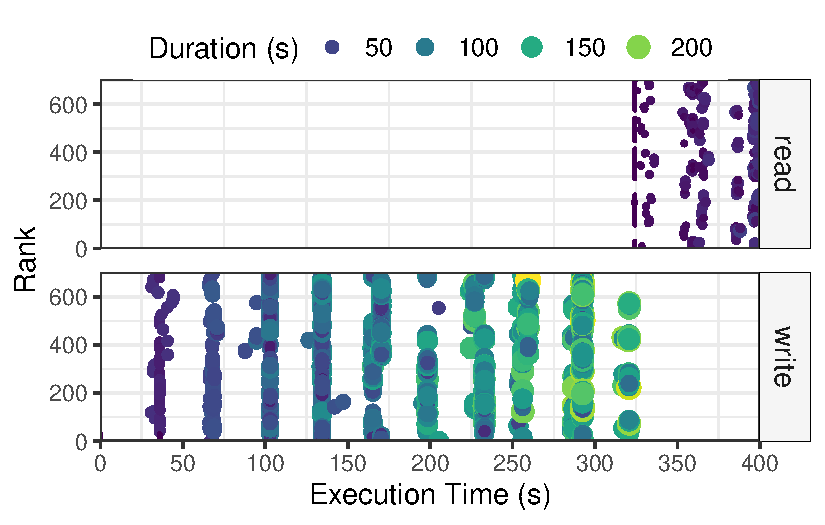
\includegraphics[width=\linewidth]{figs/255653_mpi_io_luster_no_coll_execution2.pdf}
	\caption{Distribution of read and write operations
          throughout the execution time for MPI-IO \texttt{job\_id 2},
          can reveal the application I/O pattern, and where in time, relative to the beginning
of the application execution,
          there were faster and slower operations.}
	\label{f:mpi_io}
\end{figure}
\begin{figure*}
	\centering
	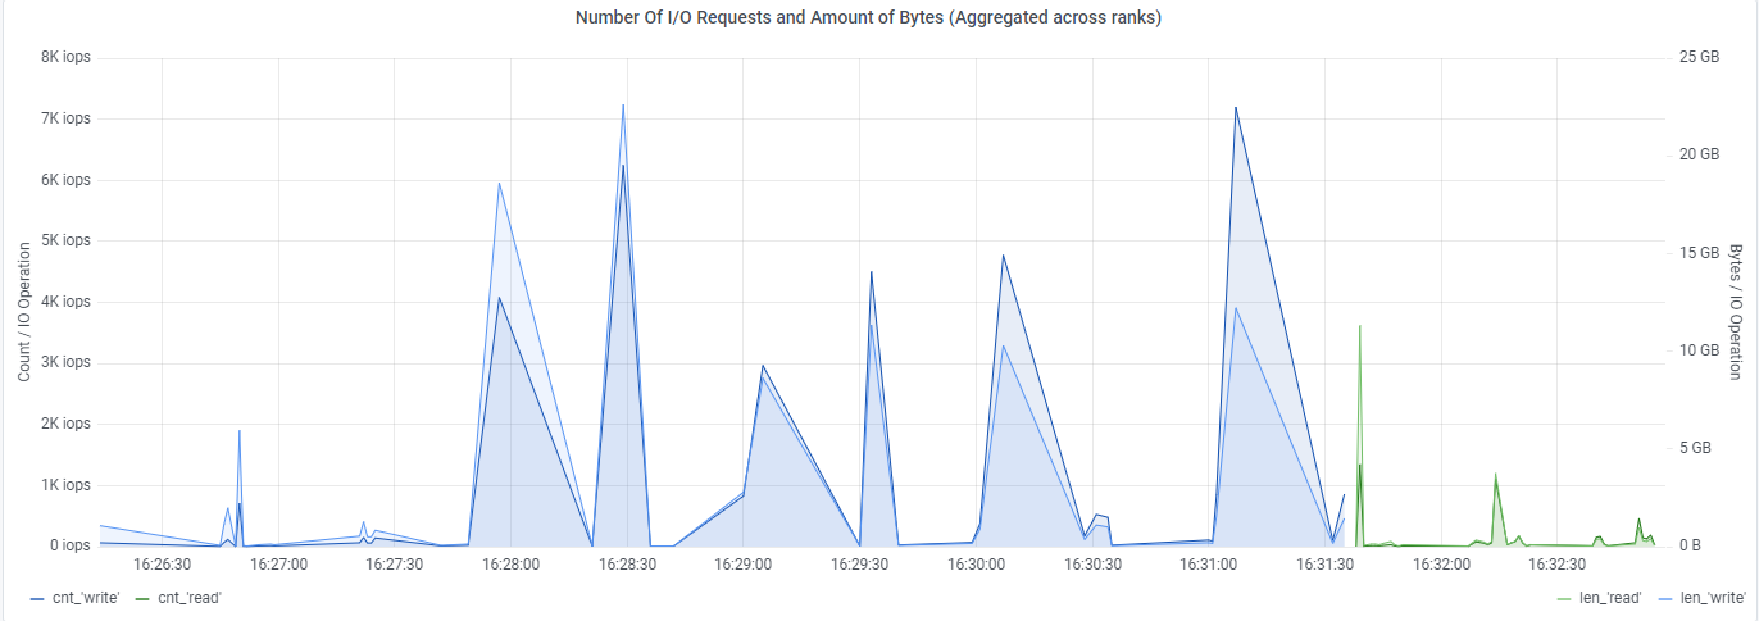
\includegraphics[width=\textwidth]{figs/255653_mpi_io_luster_no_coll.pdf}
	\caption{Graphana visualization of MPI-IO \texttt{job\_id 2}
          writes (blue) and reads (green) operations and number of bytes per
          operation, using the absolute timestamp metric collected
	  with \Darshan{}.}
	  \label{f:mpi_io_grafana}
\end{figure*}

The same job is also represented in Figure \ref{f:mpi_io_grafana}
using the Grafana interface. This figure presents an aggregate time
series across all ranks of the number of I/O
writes (blues), reads (green), and bytes sent.
This time series shows the read and write behaviors throughout execution 
time which provides further insights into I/O occurrences and size. For 
example, we can identify the two instances in which a write above 20GB 
occurs and the single instance in which a read above 10GB occurs. A developer 
or user can then use this information to create new and meaningful analyses 
about their applications I/O operations and patterns. Grafana offers an 
interactive front-end view where users can easily filter to visualize 
specific time intevals and metrics. Such representation using the absolute timestamps
facilitates the correlation of I/O performance with system component state
and behavioral characteristics (e.g., congestion in networks and filesystems)
which can also be represented in Grafana dashboards.

Without the kind of data provided by the \connector{}, it would not be possible 
to create the meaningful analyses and visualizations shown in 
Figures\ref{f:mpi_io_all}-\ref{f:mpi_io_grafana}. In contrast, 
Figure~\ref{f:hacc2} shows the aggregate I/O behavior which can be created 
with Darshan alone without the DXT plugin. This figure does not provide the 
timeseries data and thus in-depth insights into I/O behavior like the \Darshan{} does.


